\documentclass{beamer}
\usepackage[spanish]{babel}
\usepackage{graphicx}


\usetheme{default}
\usecolortheme{crane}
\beamertemplatenavigationsymbolsempty
\setbeamercovered{transparent}

\title{Prueba de Oposición Ayudante de Primera}
\author{Eric Brandwein}
\date{12 de abril de 2024}

\begin{document}

\begin{frame}
  \titlepage
\end{frame}

\begin{frame}{Programa de Técnicas de Diseño de Algoritmos}
    \begin{itemize}
        \item<1-2> Diseño y análisis de algoritmos
        \begin{itemize}
            \item<1-2> Backtracking
            \item<1-2> Programación Dinámica
            \item<1-2> Algoritmos Golosos (Greedy)
            \item<-1> Divide \& Conquer
        \end{itemize}
        \item<-1> Estructuras de Datos y Algoritmos en Grafos
        \item<-1> Algoritmos Avanzados en Grafos
        \begin{itemize}
            \item Árboles Generadores Mínimos
            \item Camino Mínimo
            \item Flujo Máximo
        \end{itemize}
    \end{itemize}
\end{frame}

\begin{frame}
    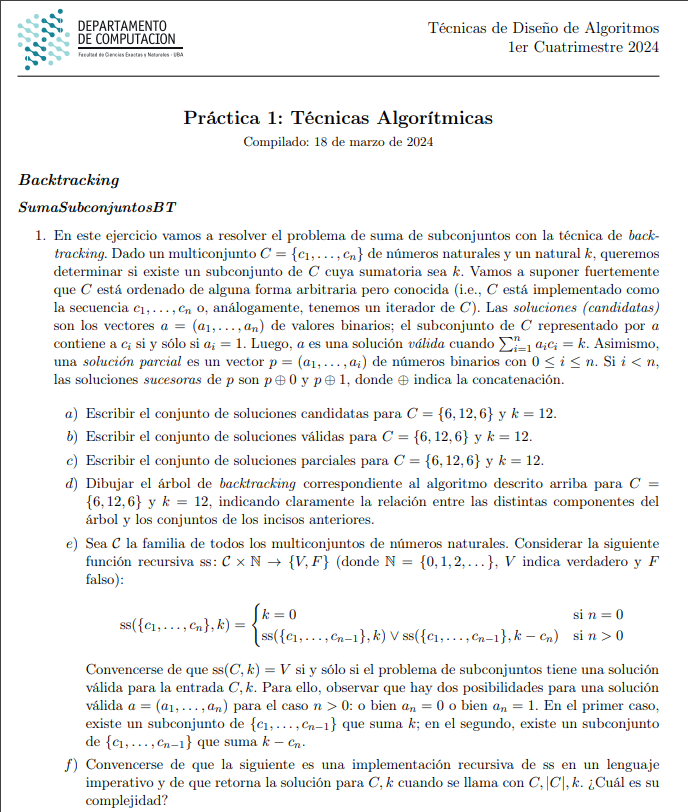
\includegraphics[trim={1mm 0 0 1mm}, clip, width=\textwidth]{img/titulo-guia.png}
\end{frame}

\begin{frame}{Objetivos}
    \begin{itemize}[<+->]
        \item Introducir técnicas sofisticadas de algoritmia.
        \item Comparar los distintos enfoques.
        \item Preparar para los siguientes temas de la materia.
    \end{itemize}
\end{frame}


\begin{frame}{Características}
    \begin{itemize}
        \item Backtracking: 4 ejercicios
        \item Programación Dinámica: 8 ejercicios
        \item Greedy: 7 ejercicios
    \end{itemize}
    + 2 ejercicios integradores = 21 ejercicios.
    \vspace{1em}

    \onslide<2-> Muchos subitems.
\end{frame}

\begin{frame}{Qué saben los alumnos}
    \begin{itemize}[<+->]
        \item Algún lenguaje de programación imperativo.
        \item Fórmulas de álgebra.
        \item Estructuras de datos.
    \end{itemize}
\end{frame}

\begin{frame}{SumaSubconjuntosBT}
    \begin{block}{Problema}
        1. Dado un multiconjunto $C$ de números naturales y un natural $k$, determinar si existe un subconjunto $S$ de $C$ tal que la suma de los elementos de $S$ sea $k$. 
    \end{block}
\end{frame}

\begin{frame}{SumaSubconjuntosBT}{Ejemplo}
    
    {\Huge 
    \begin{align*}
        C &= \{2,4,2,1\}\\
        k &= 7
    \end{align*}
    }
\end{frame}

\begin{frame}{SumaSubconjuntosBT}{Ejemplo}
    
    {\Huge 
    \begin{align*}
        C &= \{\mathcolor{red}{2},\mathcolor{red}{4},\mathcolor{red}{2},1\}\\
        k &= 7
    \end{align*}
    }
\end{frame}

\begin{frame}{SumaSubconjuntosBT}{Ejemplo}
    
    {\Huge 
    \begin{align*}
        C &= \{2,\mathcolor{green}{4},\mathcolor{green}{2},\mathcolor{green}{1}\}\\
        k &= 7
    \end{align*}
    }
\end{frame}

\begin{frame}{SumaSubconjuntosBT}{Construyendo soluciones}

    {\Huge 
    \begin{align*}
        C &= \{2,4,2,1\}\\
        k &= 7\\
        i &= 0\\
        S &= \{\}
    \end{align*}
    }
\end{frame}

\begin{frame}{SumaSubconjuntosBT}{Construyendo soluciones}

    {\Huge 
    \begin{align*}
        C &= \{\mathcolor{blue}{2},4,2,1\}\\
        k &= 7\\
        i &= 0\\
        S &= \{2\}
    \end{align*}
    }
\end{frame}

\begin{frame}{SumaSubconjuntosBT}{Construyendo soluciones}

    {\Huge 
    \begin{align*}
        C &= \{2,\mathcolor{red}{4},2,1\}\\
        k &= 7\\
        i &= 1\\
        S &= \{2\}
    \end{align*}
    }
\end{frame}


\begin{frame}{SumaSubconjuntosBT}{Construyendo soluciones}

    {\Huge 
    \begin{align*}
        C &= \{2,4,\mathcolor{blue}{2},1\}\\
        k &= 7\\
        i &= 2\\
        S &= \{2, 2\}
    \end{align*}
    }
\end{frame}

\begin{frame}{SumaSubconjuntosBT}{Construyendo soluciones}

    {\Huge 
    \begin{align*}
        C &= \{2,4,2,\mathcolor{blue}{1}\}\\
        k &= 7\\
        i &= 3\\
        S &= \{2, 2, 1\}
    \end{align*}
    }
\end{frame}

\begin{frame}{SumaSubconjuntosBT}{Fórmula recursiva}
    \begin{multline*}
        \text{haySubconjunto}(C, i, k) = \\\begin{cases}
            k == 0 & \text{si } i = |C|\\
            \text{haySubconjunto}(C, i+1, k - C[i]) \lor \\\quad\text{haySubconjunto}(C, i+1, k)  & \text{sino}
        \end{cases}   
    \end{multline*}
\end{frame}

\begin{frame}{SumaSubconjuntosBT}{Podas}
    ¿Qué pasa si $k = 0$ antes de llegar al final?
    \vspace{1em}

    \onslide<2-> ¿Y si $k < 0$?
    \vspace{1em}

    \onslide<3-> ¿Hay forma de saber con antelación que \textbf{no} vamos a poder llegar a una solución?
\end{frame}

\begin{frame}{SumaSubconjuntosBT}{Fórmula recursiva (con podas)}
    \begin{multline*}
        \text{haySubconjunto}(C, i, k) = \\\begin{cases}
            \mathcolor{blue}{Verdadero & \text{si } k = 0}\\
            \mathcolor{blue}{Falso & \text{si } k < 0}\\
            Falso & \text{si } i = |C| \land k \neq 0\\
            \mathcolor{blue}{Falso & \text{si } \sum_{j=i}^{|C| - 1} C[j] < k}\\
            \text{haySubconjunto}(C, i+1, k - C[i]) \lor \\\quad\text{haySubconjunto}(C, i+1, k)  & \text{sino}
        \end{cases}   
    \end{multline*}
\end{frame}

\begin{frame}

    \centering{\Huge  ¡Gracias!}
    
\end{frame}
\end{document}
